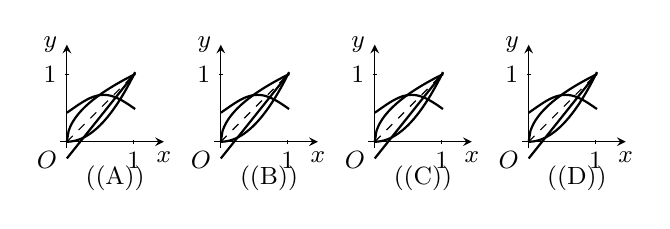
\begin{tikzpicture}[>=stealth, scale=0.85]
  % 四个候选图象：均画在 (0,1) 上，虚线为 y=x
  \foreach \dx/\name/\kind in {0/(A)/above, 2.3/(B)/below, 4.6/(C)/crossover, 6.9/(D)/crossunder}{
    \begin{scope}[shift={(\dx,0)}]
      \draw[->] (-0.1,0) -- (1.45,0) node[below] {\small $x$};
      \draw[->] (0,-0.1) -- (0,1.45) node[left] {\small $y$};
      \node[below left] at (0,0) {\small $O$};
      \draw[dashed] (0,0) -- (1.05,1.05);
      \draw (-0.03,1) -- (0.03,1) node[left=1pt] {\small $1$};
      \draw (1,-0.03) -- (1,0.03) node[below=1pt] {\small $1$};
      \ifthenelse{\equal{\kind}{above}}{%
        \draw[thick, domain=0:1.02, samples=40] plot (\x,{sqrt(\x)});%
      }{%
      \ifthenelse{\equal{\kind}{below}}{%
        \draw[thick, domain=0:1.02, samples=40] plot (\x,{\x*\x});%
      }{%
      \ifthenelse{\equal{\kind}{crossover}}{%
        \draw[thick, domain=0:1.02, samples=40] plot (\x,{1.25*\x - 0.25});%
      }{%
        \draw[thick, domain=0:1.02, samples=40] plot (\x,{0.55*exp(-2.2*(\x-0.55)^2)+0.15});%
      }}}%
      \node[below] at (0.72,-0.22) {\small (\name)};
    \end{scope}
  }
\end{tikzpicture}
